\documentclass{article}
\usepackage{graphicx} % Required for the inclusion of images
\usepackage{natbib} % Required to change bibliography style to APA
\usepackage{amsmath} % Required for some math elements 
\usepackage{wrapfig}
\usepackage{libertine} 
\usepackage{float}
\usepackage{listings}
\usepackage[skip=4pt]{caption}
\usepackage{float}
\usepackage[a4paper, margin=1in]{geometry}
\usepackage{subfig}
\setlength\parindent{0pt} % Removes all indentation from paragraphs

\renewcommand{\today}{\ifcase \month \or January\or February\or March\or %
April\or May \or June\or July\or August\or September\or October\or November\or %
December\fi, \number \year} 
\renewcommand{\labelenumi}{\alph{enumi}.} % Make numbering in the enumerate environment by letter rather than number (e.g. section 6)

%\usepackage{times} % Uncomment to use the Times New Roman font

\title{Neural Networks and Deep Learning \\ Homework 2: Unsupervised Deep Learning}

\author{Giulio \textsc{Zani}} % Author name

\begin{document}

\maketitle

\tableofcontents

\section{Introduction}
In this homework we were asked to explore unsupervised deep learning models. I have choosen to work with the MNIST dataset, as in homework 1. Yet this time, during training, I have ignored the labels of the dataset. 
\begin{figure}[H]
  \begin{center}
    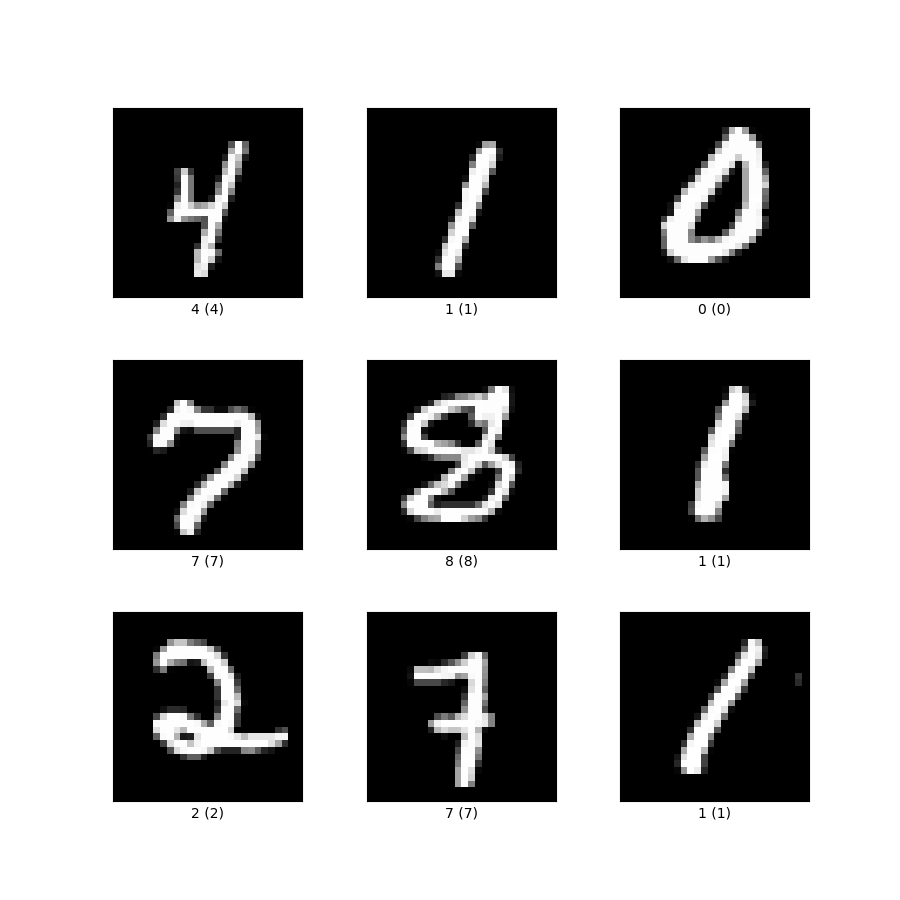
\includegraphics[width=10cm]{imgs/mnist_raw_data.png}
    \caption{Some examples of MNIST images}\label{mnist_raw_data}
  \end{center}
\end{figure}

Besides training and parameters fine-tuning, we were asked to perform these tasks:
\begin{itemize}
  \item Implement and test denoising autoencoders
  \item Fine-tune the (convolutional) autoencoder using a supervised classification task
  \item explore the latent space structure (e.g., PCA, t-SNE) and generate new samples from latent codes
\end{itemize}
Unfortunately due to time contraints I did not perform the second subtask: fine-tuning witha a supervised task.


\section{Method}

When I first learned abouit variational autoencoders (VAEs) I was charmed by them and thus decded to use them for this project. I started out from an example I have found on the internet and then improved it to finally get to the convolutional variational autoencoder I have used for this task.

This is the network structure blueprint:
\begin{lstlisting}
ConvVAE(
  (conv): Conv2d(1, 32, kernel_size=(3, 3), stride=(1, 1))
  (fc21): Linear(in_features=21632, out_features=20, bias=True)
  (fc22): Linear(in_features=21632, out_features=20, bias=True)
  (fc3): Linear(in_features=20, out_features=21632, bias=True)
  (t_conv): ConvTranspose2d(32, 1, kernel_size=(3, 3), stride=(1, 1))
)
\end{lstlisting}
In the above blueprint conv, fc21 and fc22 are part of the encoder structure, whereas fc3 and t\_conv (transpose convolution) are part of the decoder. 
I have used \textbf{ReLU} activation function and \textbf{Adam} optimizer. Training was performed for 30 epochs.

\subsection{Optimizing Hyperparameters with Genetic Algorithm}
I have used the same genetic optimization tool I created for homework 1 to optimize hyperparameters in this task. As done previously to compute hyperparameters' fitness I ran the model for one epoch and computed the test loss. I ran it with a population size of 30 and for 12 generations. The hyperparameters and their ranges are the following:

$$
\textrm{batch size} \in \{10,...,128\}
$$
$$
\textrm{lr} \in [1e-8, 1.0]
$$
$$
\textrm{gamma} \in [0, 1.0]
$$
$$
\textrm{weight decay} \in [1e-7, 1e-4]
$$

The evolved hyperparameters are:
$$
\textrm{batch size} = 49
$$
$$
\textrm{lr} = 0.428
$$
$$
\textrm{gamma} = 1.0
$$
$$
\textrm{weight decay} = 3.2318e-05
$$

With more time and computational resources it would have been interesting to explore network structure optimization.

\subsection{Training and network analysis}
\begin{figure}[H]%
    \centering
    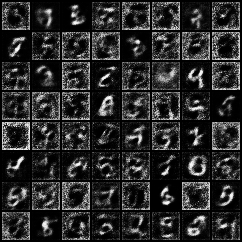
\includegraphics[width=7cm]{imgs/sample_1.png}
    \subfloat{{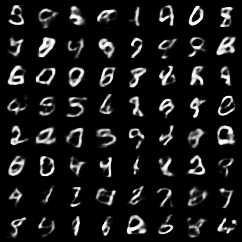
\includegraphics[width=7cm]{imgs/sample_15.png} }}
    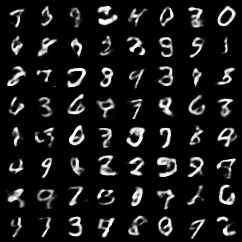
\includegraphics[width=7cm]{imgs/sample_30.png}
    \caption{Sampling after 1 (upper most) 15 (left) and 30 (right) epochs.}%
    \label{samples}%
\end{figure}
\begin{figure}[H]%
    \centering
    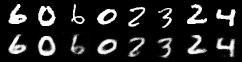
\includegraphics[width=9cm]{imgs/reconstruction_1.png}
    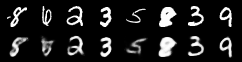
\includegraphics[width=9cm]{imgs/reconstruction_15.png}
    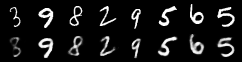
\includegraphics[width=9cm]{imgs/reconstruction_30.png}
    \caption{Reconstruction after 1, 15 and 30 epochs}%
    \label{recontruction}%
\end{figure}

\subsection{Denoising}
I have tried adding some noise to original MNIST images and checked the quality of the images output from the network:
\begin{figure}[H]
  \begin{center}
    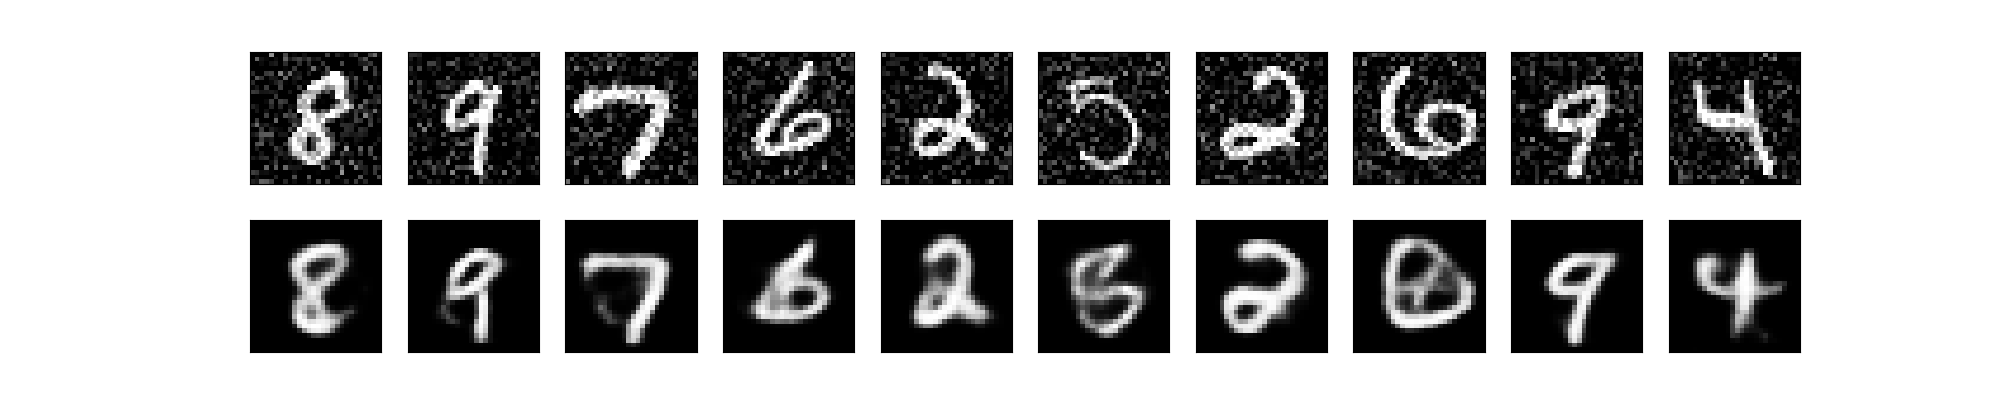
\includegraphics[width=\linewidth]{imgs/denoise.png}
    \caption{Random noise added to MNIST images (above) and its VAE output (below)}\label{denoise}
  \end{center}
\end{figure}
Results were interesting but far from perfect, for example a five was turned into an eight.

\subsection{PCA of latent structure}
I did the following: for each of the 20000 images I've choosen to pick for this task, I encoded it, then reparametrised and finally performed a 2-dimension PCA of the resulting matrix. I have used the PCA implementaion of the sklearn package.
\begin{figure}[H]
  \begin{center}
    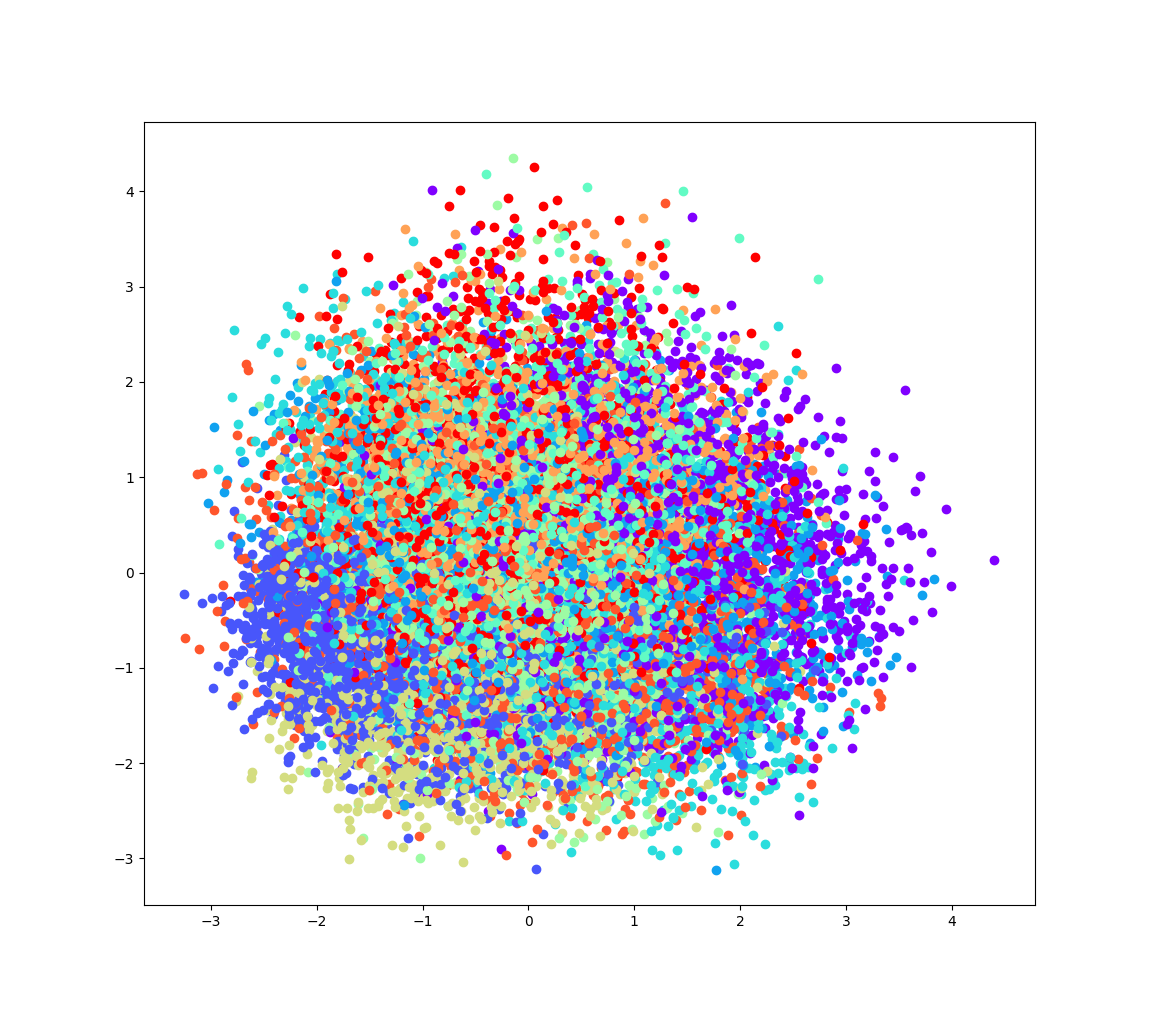
\includegraphics[width=\linewidth]{imgs/pca_latent_space.png}
    \caption{PCA of the network's latent space, sampled using 20000 images. Different colors represent the different labels (0 to 9)}\label{pca}
  \end{center}
\end{figure}

As one can see in \figurename{\ref{pca} some clusters are visible, but they're very fuzzy and they overlap with each others. There appear to be colors, i.e., digits which don't have clusters. Perhaps this is due to suboptimal learning or due to too low dimensionality pca. I have also tried performin a 3 dimensional PCA with a similar procedure, using 2000 images (see \figurename{\ref{3d_pca}}).

\begin{figure}[H]
  \begin{center}
    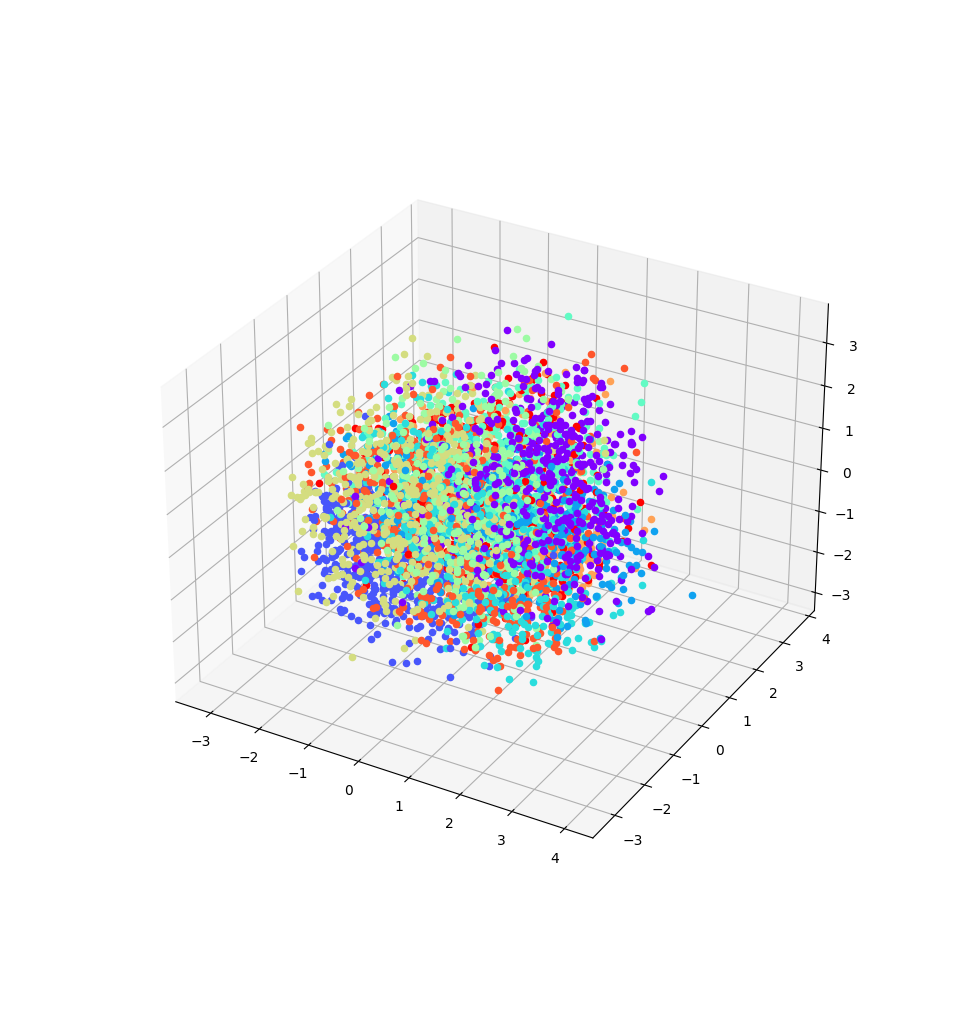
\includegraphics[width=\linewidth]{imgs/3D_PCA.png}
    \caption{3 dimentional PCA of the network's latent space, sampled using 2000 images. Different colors represent the different labels (0 to 9)}\label{3d_pca}
  \end{center}
\end{figure}


\begin{lstlisting}
python -m deep_learning_hw2
\end{lstlisting}


\section{Result}
The test loss of the trained model is 100.9932

\end{document}
